\documentclass[fleqn,a4paper,12pt,titlepage,headsepline]{scrartcl}

\usepackage{gauss} 
\usepackage{fancyhdr}


\usepackage[footskip=30pt]{geometry}

\usepackage{bm}
%für dicke Buchstaben im Mathemodus

\usepackage{bigints}

\usepackage{ziffer}

\usepackage[T1]{fontenc}
%das ist für europäische Zeichen

\usepackage[utf8]{inputenc}
%das ist für Sonderzeichen

\usepackage{rotating}
\usepackage{multirow}
\usepackage{tabularx}
\usepackage{longtable}

\usepackage{booktabs}

\usepackage{lmodern}
%das ist für Umlaute

\usepackage[ngerman]{babel}
%das ist für deutsche Sprache


\geometry{
	left=1.5cm,
	right=1.5cm,
	top=1cm,
	bottom=.5cm,
	bindingoffset=5mm
}


\usepackage{graphicx}
%für Bilder


\usepackage{graphicx}
\usepackage{float}

\usepackage[center]{caption}

\usepackage{wrapfig}



\linespread{1.25}

\pagestyle{fancy}
\fancyhf{}
\fancyhead{ }
\fancyhead{ }
\fancyfoot{von Gabriela }


\begin{document}
	\begin{center}
	\begin{huge}
	\noindent Lösung
	\end{huge}
	\end{center}
\noindent \textbf{Hinweis:}
Die Phasen sind zyklisch und werden von links nach rechts gelesen.
\begin{center}
					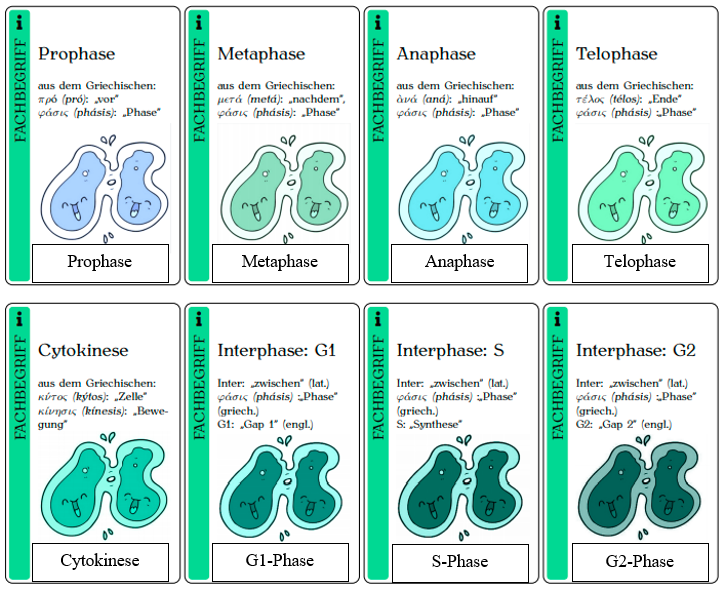
\includegraphics[scale=0.81]{fachbegriff.png} 				\end{center}
	\begin{center}
					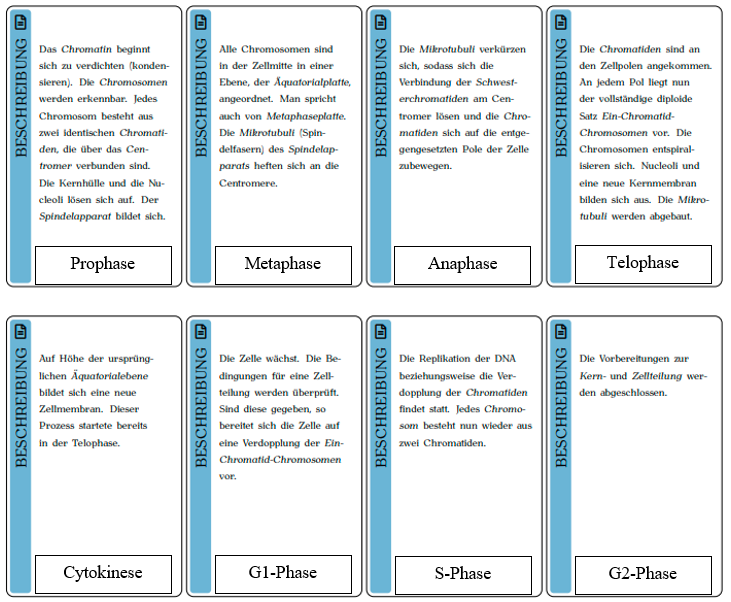
\includegraphics[scale=0.81]{beschreibung.png} 				\end{center}
	\begin{center}
					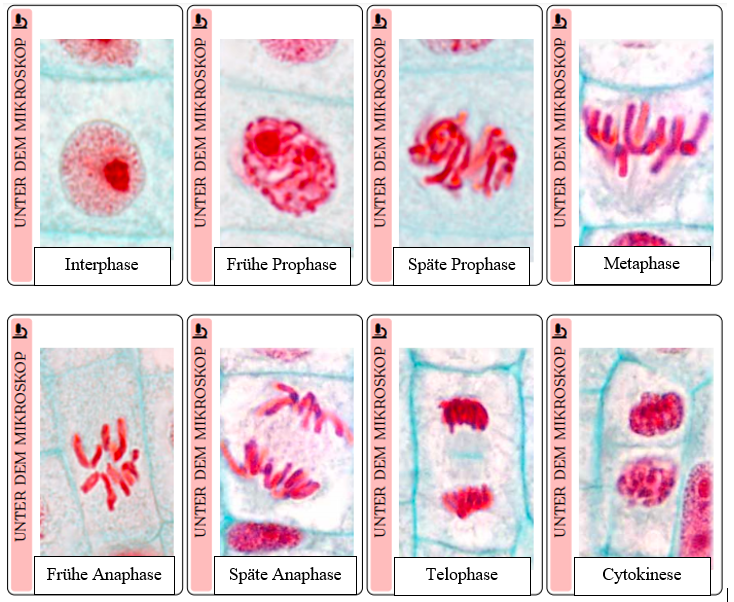
\includegraphics[scale=0.81]{mikroskop.png} 				\end{center}	
	\begin{center}
					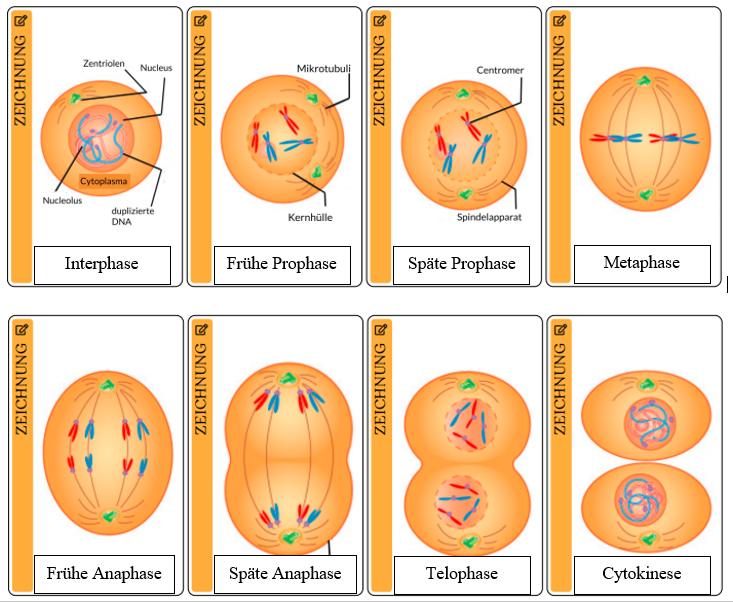
\includegraphics[scale=0.81]{skizze.png} 				\end{center}
\newpage

	\end{document}